\clearpage
\section{Heat Diffusion}
\begin{colbox}
	\begin{enumerate}
		\item What are the dimensional quantities in the problem? What are their dimensions? Separate your answer into parameters, dependent variables, and independent variables.
		\item Find 2 dimensionaless combinations. Using them, write a self-similar solution, as we saw in the tutorial. Does your solution satisfy the boundary conditions?
		\item Substitute the solution into the heat equation to obtain a second-order ordinary differential equation.
		\item Solve the equation. What is the boundary condition at \(x\rightarrow\infty\)?
		\item Plot the temperature distribution along the rod at different times?
	\end{enumerate}
\end{colbox}
\subsection{Dimensions}
The dimensional parameter in this problem are \(k\) the thermal diffusion coefficient with dimensions \(L^2 t^{-1}\) and \(T_0\) which has dimensions of \(TL\) where T is temperature and L is length. The independent variables are \(x\) which has dimensions of length and \(t\) which has dimension of time. The dependent variable in the problem is the temperature at each point, which has dimensions of temperature.
\subsection{Dimensionless combinations}
Similarly to the training we can define
\begin{align}
	\xi = \frac{x}{\sqrt{kt}} = x\ins{kt}^{-1/2} && \theta = \frac{T}{T_0}
\end{align}
Which then gives us the self-similar solution
\begin{equation}
	\theta = \Phi(\xi) \rightarrow T = T_0\Phi(\xi)
\end{equation}
We require new boundary conditions:
\begin{align}
	\Phi(0)=1 && \Phi(x\rightarrow\infty)=0
\end{align}
\subsection{Inserting Solution}
Rewriting the left hand side first:
\begin{align}
	\del{t}T &= T_0 \del{t}\Phi(\xi) = T_0 \pdv{\Phi}{\xi}\pdv{\xi}{t} = -\frac{xT_0}{2k^{-1/2}t^{-3/2}}\pdv{\Phi}{\xi} = -\frac{\xi T_0}{2t}\pdv{\Phi}{\xi} \\
	\del{x}T &= T_0\del{x}\Phi=T_0\pdv{\Phi}{\xi}\pdv{\xi}{x} = \frac{T_0}{\sqrt{kt}}\pdv{\Phi}{\xi}
\end{align}
therefore the equation becomes
\begin{equation}
	-\frac{\xi T_0}{2t}\pdv{\Phi}{\xi} = \frac{kT_0}{kt}\pdv[2]{\Phi}{\xi}
\end{equation}
rearranging to
\begin{equation}
	\pdv[2]{\Phi}{\xi}+\frac{\xi}{2}\pdv{\Phi}{\xi}=0
\end{equation}
which is indeed a second order ordinary differential equation.
\subsection{Solving}
Using the hint the solution is
\begin{equation}
	\Phi = A\erf(\frac{\xi}{2})+B
\end{equation}
Using the boundary condition that \(\Phi(\xi=0)=1\) we find that \(B=1\). Using the boundary condition that \(\Phi(x\rightarrow\infty)=0\) we find that \(A=-1\). Therefore the solution is
\begin{equation}
	\Phi(\xi) = 1-\erf(\frac{\xi}{2})
\end{equation}
And the original equation's solution is
\begin{equation}\label{thesolution}
	T = T_0\ins{1-\erf(\frac{\xi}{2})}
\end{equation}
\subsection{Plot}
\begin{figure}[!htb]
	\centering
	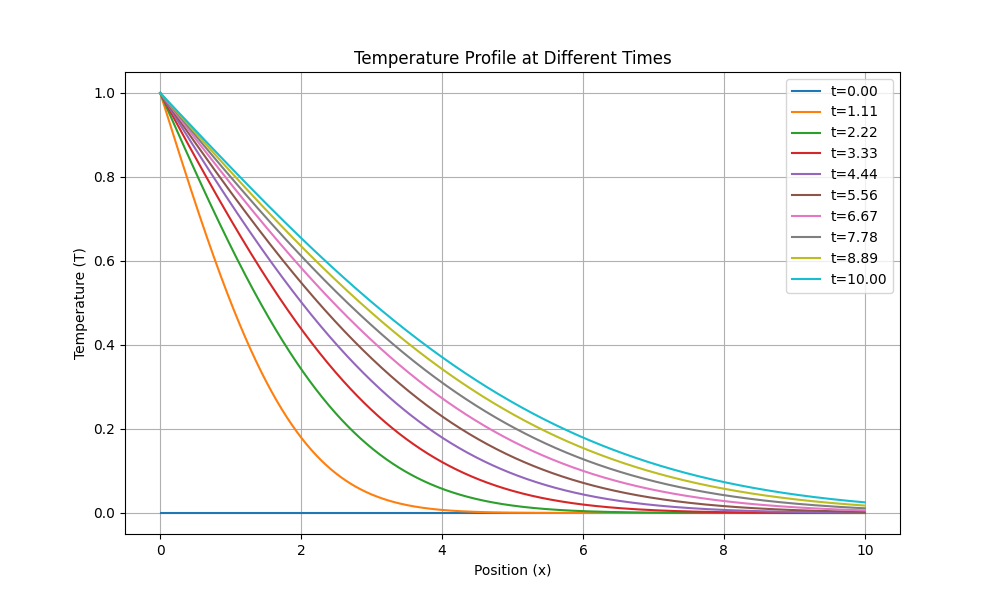
\includegraphics[width=0.9\textwidth]{Figure_1.png}
	\caption{The temperature profile along the x axis of the rod at different times, as given by equation \ref{thesolution}.}
\end{figure}
\newpage
\begin{lstlisting}[language=Python, caption=The code]
import matplotlib.pyplot as plt
import numpy as np
from scipy.special import erf

def plot_profile_at_times(times, x, T):
    plt.figure(figsize=(10, 6))
    for t in times:
        plt.plot(x, T(x, t), label=f't={t:.2f}')
    plt.xlabel('Position (x)')
    plt.ylabel('Temperature (T)')
    plt.title('Temperature Profile at Different Times')
    plt.legend()
    plt.grid()
    plt.show()

def main():
    # temperature and coefficient are both assumed to be 1 for simplicity
    # the position also isn't really the real position, scaling will be off
    # but I imagine it's not very important for this.
    held_temp = 1
    xi = lambda x,t: x/np.sqrt(t)
    solution = lambda x,t: held_temp*(1-erf(xi(x,t)/2)) 
    times = np.linspace(0, 10, 10)
    x = np.linspace(0, 10, 1000)
    plot_profile_at_times(times, x, solution)

if __name__ == "__main__":
    main()
\end{lstlisting}